\chapter{Optimising Contur}
\label{chapterlabel5}
In this section we will outline the optimisation changes made to \textbf{Contur} as part of this research project. Our focus will be on optimising the grid run, mainly because for research purposes users will in general be spending most of their time running \textbf{Contur} on a grid as opposed to single \textbf{YODA} files. So focusing our optimisation efforts on the grid run is likely to produce more practical benefits for users. In addition we have two other motivations for focusing our efforts on optimising the grid run:

\begin{itemize}
\item There is more scope for achieving meaningful improvements in runtime with the grid run. This viewpoint comes from observing from figure \ref{fig:single_yoda_start_profile_snakeviz} that the single \textbf{YODA} runtime only takes around $20$ seconds, while from figure \ref{fig:grid_yoda_start_profile} we can see that the runtime for a smallish grid\footnote{The grid we are profiling is $10 \times 10$, so contains $100$ \textbf{YODA} files, for research purposes it is common to run such a $10 \times 10$ grid across three different energy buckets ($7$,$10$ and $13$ TeV), with each bucket having $100$ \textbf{YODA} files for a total of $300$. So the $20$ minutes we profiled for a single $10 \times 10$ grid would likely be close to an hour if run across the three energy buckets} takes up to $20$ minutes. Thus decreasing runtime for the single \textbf{YODA}  by $50\%$ will only save us $10$ seconds in absolute terms, while the equivalent decrease for the grid run would save us $10$ minutes\footnote{Or $30$ minutes for the case where the grid has three energy buckets.};
\item There is more scope for the grid runtime to increase with changing research needs. The grid runtime is dependent on the size of the grid, as the grid grows in size the runtime will increase. There is a practical limit to how big a grid can be resulting from this increasing runtime, in effect once a grid is so large it is too slow to run on. Optimisations to the grid run that not only improve runtime on the current standard size grids but also reduce the speed that runtime increases with increasing grid size could have very practical benefits like making runs feasible on large grids where previously the run time was too slow;
\end{itemize}

For the above reasons the main focus of the optimisation from here on in will be on the grid run. From the dot plot in figure \ref{fig:grid_yoda_start_profile_dot} arising from the data produced from our initial grid profile we can see that grid runtime arises from two branches in the code flow, the first arising from the \texttt{sort\_blocks()} method\footnote{See dark green box in dot plot}, which takes c.a. $25\%$ of runtime and the second being the calculation of the $CL_s$ exclusions for each histogram\footnote{sequence of boxes in the dot plot starting as yellow and morphing to green} which takes most of the remainder runtime. Our initial efforts will focus on making optimisation improvements for these two parts for the program.

\section{Sort Blocks Method}\label{sortBlocksSection}

\subsection{Background}
In section \ref{calculate_likelihood} we gave a brief overview into how \textbf{Contur} calculates the $CL_s$ exclusion for a single passed \textbf{YODA} file. Additionally we also  highlighted the similarities between the single \textbf{YODA} and the grid runs. We will now go into a bit greater detail to give the necessary background to understand the optimisation change covered in this section.

\textbf{Contur} contains three main classes to coordinate a run, the \classname{depot} class, \classname{yoda\_factories} and the  \classname{likelihood} class. The \classname{depot} class deals with the overall control of a run and is where all results are stored, while the \classname{likelihood} class calculates the $CL_s$ exclusion for each histogram. The \classname{yoda\_factories} class sits between these two classes in the flow of a run. Each \textbf{YODA} file that the \classname{depot} object finds in a grid gets passed to \classname{yoda\_factories}. Upon instantiation of a \classname{yoda\_factories} object with a  \textbf{YODA} file, \classname{yoda\_factories} gathers all necessary data\footnote{This consists of both the simulated data contained in the passed \textbf{YODA} file and experimental data from \textbf{Rivet}}, and then for each histogram in the passed  \textbf{YODA} file, \classname{yoda\_factories} instantiates a \classname{likelihood} object to calculate the $CL_s$ exclusion for the histogram. The end result of instantiating \classname{yoda\_factories} is that its \texttt{likelihood\_blocks} attribute will contain a list of the \classname{likelihood} objects instantiated for each histogram. Each of these \classname{likelihood} objects will contain the $CL_s$ for a histogram as an attribute.

The \texttt{sort\_blocks()} method of \classname{yoda\_factories} is called after an object has been instantiated and the \texttt{likelihood\_blocks} attribute has been populated. The method takes the list of \classname{Likelihood} objects in the \texttt{likelihood\_blocks} list and buckets the \classname{Likelihood} objects into pools. After this bucketing for each pool the method then finds the \classname{Likelihood} object in each pool with the largest $CL_{s}$, the selected \classname{Likelihood} objects are used to create a new list of \classname{Likelihood} objects which are stored in \classname{yoda\_factories} \texttt{sorted\_blocks} attribute.

\subsection{Changes made}
The profiling results in the dot plot in figure  \ref{fig:single_yoda_start_profile_snakeviz} are precise enough that we can pin point the major slow point in the \texttt{sort\_blocks()} method to be the list comprehension in line $958$ of \classname{yodafactories}\footnote{This can also be easily picked up in the icicle plot when using Snakeviz's graphical viewer}. This list comprehension sits within a loop and the whole block of code can be seen in listing \ref{code:sort_blocks_list_comprehension} below.

\begin{code}
\captionof{listing}{Sort Blocks List Comprehension}
\label{code:sort_blocks_list_comprehension}
\begin{minted}{python}
for p in pools:
  if not p == omitted_pools:
    for item in l_blocks:
      if item.CLs == 
         max([x.CLs for x in l_blocks if x.pools == p]) 
\end{minted}
\end{code}

In the above block of code the list comprehension in the last line is used to find the \classname{Likelihood} object in each pool with the largest $CL_s$. The list comprehension on its own is not particularly slow, it is however  placed within a nested for loop, which loops over pools and then within each pool iterate we have another loop over the \texttt{likelihood\_blocks} list. So in each \textbf{YODA} file the number of times listing \ref{code:sort_blocks_list_comprehension} is called is given by the number of pools multiplied by the length of the \texttt{likelihood\_blocks} list. While over a whole grid of 100 \textbf{YODA} files we will effectively be multiplying this number again by 100. Figure \ref{fig:list_comprehension} below shows that for our $10\times 10$ grid we are calling listing \ref{code:sort_blocks_list_comprehension} over a million times. So although each comprehension on its own takes less than $0.002$ seconds this multiplied by a million still gives us a run time of over $200$ seconds.  

\begin{figure}[H]
\centering
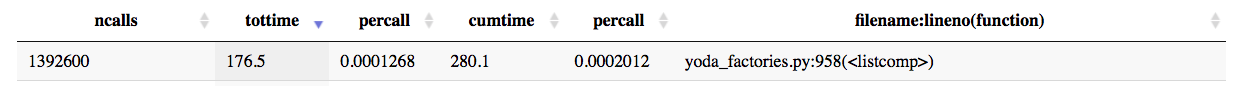
\includegraphics[scale=0.3]{plots/sort_blocks_list_comprehension.png}
\caption{List comprehension in sort blocks - Run time info}
\label{fig:list_comprehension}
\end{figure}

The optimisation change adopted here was to move the maximum $CL_s$ calculation for each pool performed by listing \ref{code:sort_blocks_list_comprehension} outside of the nested for loop. This change dramatically reduces the number of times the calculation is performed. In its place we now only perform the calculation once per \textbf{YODA} file\footnote{So in our $10\times 10$  grid we go from perform the calculation over 1 million times to exactly $100$ times, once for each \textbf{YODA} file in the grid} and store the results in a dictionary whose key is the pool and value is the maximum $CL_s$ for the pool. This dictionary is then used in place of the list comprehension in  listing \ref{code:sort_blocks_list_comprehension}. So within the nested for loop we have replaced a call to a list comprehension with a run time per call of $10^{-4}$ with a dictionary with a runtime per call\footnote{See \href{https://towardsdatascience.com/faster-lookups-in-python-1d7503e9cd38}{here} for profile information for Python's dictionary object} of $10^{-7}$, so the $10^6$ calls made in the loop will take $10^2$ seconds with our old implementation but only $10^{-1}$ seconds with the new implementation.

\subsection{Impact of changes}

Below we see the impact of the optimisation on the runtime for the \texttt{sort\_blocks()} method. In figure \ref{fig:sort_blocks_before} we can see that prior to optimisation the runtime of the list comprehension is in line with our expectations from the previous section with a runtime of $280$ seconds, order $10^2$ as expected and total runtime\footnote{Remember the list comprehension is only part of the sort blocks method, not the whole of it so we will have additional runtime from other parts of the method} for \texttt{sort\_blocks()} is $293$ seconds. While in figure \ref{fig:sort_blocks_after} we see that we have a post optimisation runtime of $7$ seconds for the whole of the \texttt{sort\_blocks()}method. This runtime supports the hypothesis that the runtime for calling the dictionary in place of the list comprehension is of order $10^{-1}$ seconds and additionally would suggest that the optimisation change made the calculation of the maximum $CL_s$  for each pool slightly faster too, as prior to optimisation \texttt{sort\_blocks()} had $13$ seconds of runtime outside of the list comprehension, now after optimisation total run time is just $7$ seconds. 

\begin{figure}[H]
\centering
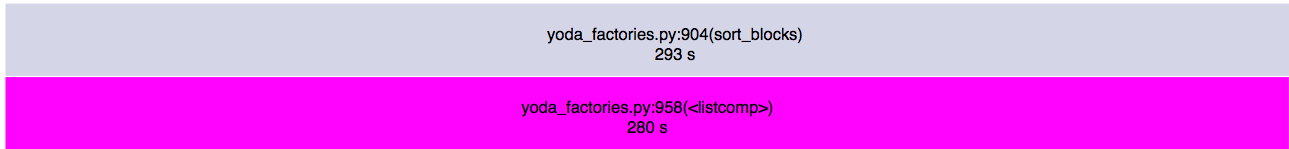
\includegraphics[scale=0.3]{plots/sort_blocks_before.png}
\caption{Sort blocks grid run time - Before optimisation}
\label{fig:sort_blocks_before}
\end{figure}



\begin{figure}[H]
\centering
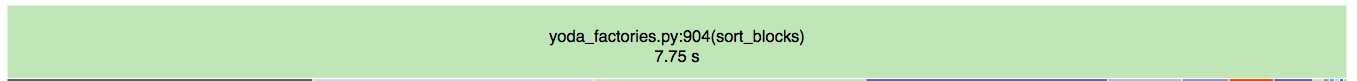
\includegraphics[scale=0.3]{plots/sort_blocks_after.png}
\caption{Sort blocks grid run time - After optimisation}
\label{fig:sort_blocks_after}
\end{figure}



\section{Likelihood Calculation}\label{sec:likelihood}
\subsection{Background}
The outlines of the workings of \textbf{Contur} to this point\footnote{See chapter \ref{chapterlabel2} Contur overview and the outline for the \texttt{sort\_blocks} method in section\ref{sortBlocksSection}} have avoided delving too deeply into how the \classname{Likelihood} object computes the $CL_s$, instead it has just been sufficient to highlight that for each histogram the calculation of the $CL_s$ takes place within the \classname{Likelihood} object. In this section we will need to delve a bit more deeply into the likelihood calculation. The reason for this comes from examining the icicle plot in figure \ref{fig:grid_yoda_start_profile}. From this plot we can that a material proportion of \textbf{Contur's} runtime is spent within the \classname{Likelihood} object\footnote{From the icicle plot we can see that out of a run time of around $1100$ seconds we spend $715$ seconds in the likelihood class calculations}.

Drilling down into the initial grid run profile results for the \classname{Likelihood} object we can see in figure \ref{fig:like_initial_profile} that the \texttt{ts\_to\_pval()} method is where most of the run time is coming from in the \classname{Likelihood} object. This method takes the test statistics which are computed by the \classname{Likelihood} object's \texttt{chisqr()} method and converts them into p-values. The test statistics are taken to have the distribution of a standard normal, so the p-value is computed just by computing the survival probability for the value of the passed test statistic. This is done using the the \classname{scipy.stats.norm} object in the Scipy library and using the \texttt{sf()} method of this object to compute the survival probability for the passed test statistic. The only function that the \texttt{ts\_to\_pval()} method in the \classname{Likelihood} object performs is to call the \texttt{sf()} method, so from this we can see that the majority of our run time in the \classname{Likelihood} object is coming from calling this one method which from here on in we will refer to as the survival function.

\begin{figure}[H]
\centering
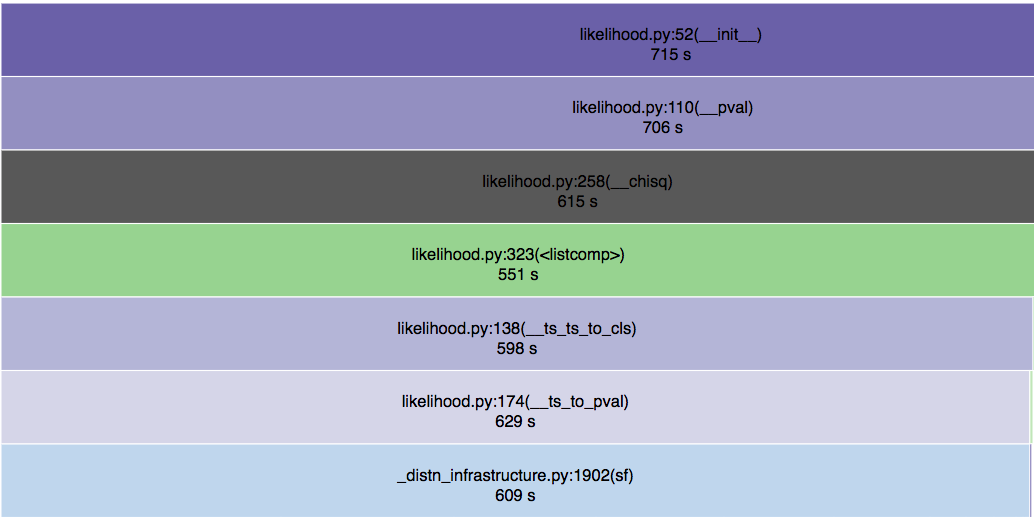
\includegraphics[scale=0.23]{plots/likelihood_drill_down.png}
\caption{Likelihood object - Initial profile}
\label{fig:like_initial_profile}
\end{figure}

From figure \ref{fig:ts_to_pval} below it becomes apparent that the large run time we observe from calling the survival function results from the large number of calls we make to the function. Each call to the survival function takes c.a. $0.0002$ seconds, but we make over $3$ million calls resulting in a total run of over $600$ seconds. 

\begin{figure}[H]
\centering
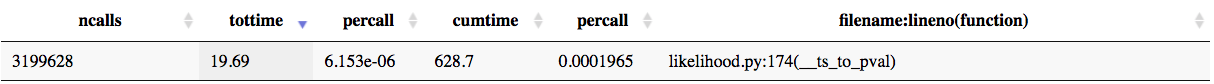
\includegraphics[scale=0.3]{plots/likelihood_count.png}
\caption{Likelihood object - ts to pval details}
\label{fig:ts_to_pval}
\end{figure}

\subsection{Scipy Normal Distribution Survival Method}
From the previous section we can conclude that greater efficiencies in the likelihood calculation can be achieved by reducing the number of times we call the survival function. It is helpful to first understand better where the calls to the survival function arise when a \classname{Likelihood} object is instantiated. Within a \classname{Likelihood} object we get calls to the survival function via the following routes:

\begin{itemize}
\item[1.] Every time the \texttt{ts\_to\_pval()} method is called we have one call to survival function. Upon instantiation this method is called twice explicitly, giving us two calls to survival function ;
\item[2.]The \texttt{ts\_ts\_to\_cls()} method calls \texttt{ts\_to\_pval()} twice internally, so every time this method is called we have two calls to the survival function. The method is called once upon instantiation giving us two more calls to the survival function.;
\item[3.] The \texttt{chisq()} method which computes the test statistics will only call the survival function when an inverse for the covariance matrix of the analysis object cannot be computed\footnote{In the code the survival function will only be called when the condition \say{self.covBuilt and sb nuisance is not None} is false}. When the method calls the survival function the number of times it makes the calls is twice the number of buckets in the analysis object. So this is a minimum of $2$ calls but potentially much more than $2$ ;
\end{itemize}

From the above we see that each histogram will have at least $4$ calls to the survival function\footnote{In practise it will be a lot more than this because of the \texttt{chisq()} calls}, so across a whole \textbf{YODA} file the number of calls to the survival function will be at least $4$ multiplied by the number of histograms in the \textbf{YODA} file\footnote{For perspective here, the $10\times 10$ grid we profiled on had c.a. 60,000 likelihood objects created across $100$ \textbf{YODA} files suggesting on average each \textbf{YODA} file had $600$ valid histograms}. Finally we have $100$ \textbf{YODA} files in our grid, which need to be summed across to give the total number of calls we make to the survival function in our grid run.

To reduce the number of calls to the survival function we will adopt two approaches. The first is simple to check if we are making any unnecessary calls to the survival function anywhere that can easily be removed, this approach is simple but will not likely give high returns. The second approach is to take greater advantage of numpy's array functionality to see if via collecting test statistics into numpy arrays and passing these arrays of test statistics to the survival function, reducing the overall number of calls\footnote{So for example if we had four test statistics we wanted to pass to the survival function we would collect the test statistics into a single array and pass the array once to the survival function as opposed to four individual calls to the survival function}.

For the second approach to be effective we require the runtime for the survival function if passed a numpy array of length $n$ to be significantly less than the runtime if we just made $n$ separate calls to the survival function. We would expect this to be the case as the survival function like all methods in Scipy is built to enable fast array based computation when passed numpy arrays. 

Figure \ref{fig:loop_v_array} below shows the result of the profile we performed to test the performance of calling the survival function $n$ times within a loop or passing an array of length $n$ once. The $x$ axis gives the value of $n$ on a log scale while the $y$ axis gives the runtime for the loop (orange line) and the array (blue line) on a log scale. So from the plot we can see that our starting profile with $n$ between $10^6$-$10^7$ should give a runtime between $10^2$-$10^3$ seconds which is in line with the c.a. $600$ seconds we actually observe.

\begin{figure}[H]
\centering
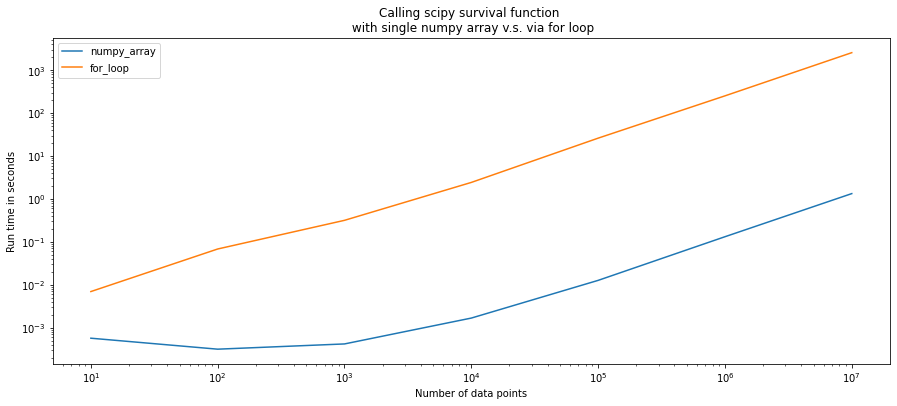
\includegraphics[scale=0.5]{plots/scipy_profile.png}
\caption{Scipy Survival Function - Loop vs Array}
\label{fig:loop_v_array}
\end{figure} 

\subsection{Changes made}
The optimisation changes to the likelihood calculation were made via multiple commits to the \textbf{Contur} repository over the space of a couple weeks, they can be grouped into three groups of changes:

\begin{itemize}
\item[1.] Within \classname{Likelihood} objects making use of numpy arrays to reduce the number of calls to the survival function;
\item[2.] Within \classname{Likelihood} objects reducing unnecessary calls to the survival function;
\item[3.] Across \classname{Likelihood} objects, use numpy arrays to reduce the number of calls. So try to gather test statistics for multiple \classname{Likelihood} objects across the \textbf{YODA} file together and make a single call to the survival function.
\end{itemize}

Of the above changes the first two are least disruptive in terms of their impact in the overall flow of a run as they only make changes within the \classname{Likelihood} class. While the third change is more substantial structural alternation to flow of a run between \classname{yoda\_factories} and the \classname{Likelihood} class.

The first change\footnote{The change can be found in commit \href{https://gitlab.com/hepcedar/contur/-/commit/0b80789580cd0529bfdce28d2bae252755c45a63}{0b807895}} involves passing a list of tuples of the background and signal test statistics to the \texttt{ts\_to\_pval()} method and to the \texttt{ts\_ts\_to\_cls()} method, as opposed to passing the test statistics as separate calls. This reduces the calls to the survival function for these values from $4$ to $2$. Listing \ref{code:single_to_tuple} below gives an example of this change, we can see when we pass the list containing the tuple we only need to call \texttt{ts\_to\_pval()} once as opposed to twice, which means we see a similar reduction in the number of times we call the survival function.
\begin{code}
\captionof{listing}{Sort Blocks List Comprehension}
\label{code:single_to_tuple}
\begin{minted}{python}
## Passing individual test statistics (before)
p_val_background = ts_to_pval(ts_background)
p_val_signal = ts_to_pval(ts_signal)

##Passing list of tuples (after)
list_ts = [(ts_background,ts_signal)]
p_val_background , p_val_signal = ts_to_pval(list_ts))

\end{minted}
\end{code}
This change also has impact within the \texttt{chisq()} method, where we also now pass a list of tuples containing the test statistics as opposed to making separate calls to the survival function. This ensures that whenever the \texttt{chisq()}  method makes a call to the survival function it only makes $1$ call, so after all these changes, for a histogram we get at least $2$ calls to the survival function and at most $3$.

The second change\footnote{The change can be found in commit \href{https://gitlab.com/hepcedar/contur/-/commit/15ef923de401ced56f3186ed3bf6528c7d46f890}{15ef923d}} made is motivated from the observation that the \texttt{ts\_ts\_to\_cls()} method has a call to \texttt{ts\_to\_pval()} within it, so it computes the p-value within the call. This is unnecessary as we have already computed the p-value. The change introduces the \texttt{pval\_to\_cls()} method which directly takes a p-value and computes the $CL_s$ from it. Negating the need to make another call to the survival function, so after this change we now have a minimum of $1$ call to the survival function and a maximum of $2$ in each histogram.

From here on in let us simplify and assume that we have exactly $2$ calls to the survival function for each histogram and for each \textbf{YODA} file we have $m$ histograms. So in a grid with $n$ \textbf{YODA} files after the above changes we have $2\times n\times m$ calls to the survival function. So for our $100$ \textbf{YODA} file grid assuming $m=600$ this will still give us 120,000 calls to the survival function. Additionally we can see with an expanding grid size this number of calls will grow, for example with 1,000 \textbf{YODA} files the number of calls to the survival function will be above 1 million again. So the current configuration is not robust against future increases in grid size. The final set of optimisation changes we will make resolves this issue by getting rid of the runtime dependence on the number of histograms $m$ per \textbf{YODA} file.

To achieve this, let us first remind ourselves how the current set up works. Upon instantiation of the \classname{yoda\_factories} class we loop through all histograms instantiating a \classname{likelihood} object for each and doing the full likelihood calculation (i.e. computing the $CL_s$) upon instantiation of the \classname{likelihood} class. So at the end of this process we have a \classname{yoda\_factories} object with a \texttt{likelihood\_blocks} attribute that contains all the \classname{likelihood} objects. This process can be split into steps that allows us to eliminate dependence on the number of histograms. This can be done by instead of using the survival function within the \classname{likelihood} object, we can instead just collect test statistics in the \classname{Likelihood} object which can then be collected into a numpy array in \classname{yoda\_factories} composed of test statistics from all the \classname{likelihood}  objects, this array can then be passed once to the survival function.

Implementing this change in practise is spread across two commits\footnote{The first commit \href{https://gitlab.com/hepcedar/contur/-/commit/299b03a86812b47e30ed66d4f82a59a3584cf523}{299b03a8} introduces the \texttt{likelihood\_blocks\_ts\_to\_cls()} function, while the second commit \href{https://gitlab.com/hepcedar/contur/-/commit/2769e1c2a020efd2de2919db2413309eef8a8e64}{2769e1c2} introduces the \texttt{likelihood\_blocks\_find\_dominant\_ts\_function()}}. For the first commit we introduce the \texttt{likelihood\_blocks\_ts\_to\_cls()} function, which takes a list of \classname{likelihood} objects and computes a $CL_s$ for each \classname{likelihood} object in the list. In terms of the flow of the run, with this change we alter the \classname{likelihood} object so it no longer calculates the $CL_s$ upon instantiation, so when we instantiate \classname{yoda\_factories} we now have a list of \classname{likelihood} objects in the l\texttt{likelihood\_blocks} attribute where each \classname{likelihood} object just contains a test statistic, we pass this list to the new function which does the confidence level calculation. After this change we will have $n + (n\times m)$ calls to the survival function.

For the second commit we introduce the \texttt{likelihood\_blocks\_find\_dominant\_ts\_function}. This function finds the test statistic in a histogram that gives the largest $CL_s$ when the covariance matrix does not have a valid inverse. Thus it moves the calls to the survival function that take place within the \texttt{chisq()} method into a single call in \classname{yoda\_factories}. After this change the number of calls to the survival function will be $2n$ so we have removed the dependence on $m$ of the number of calls. The impact of this third change in terms of the overall structure of \textbf{Contur} can be seen in listing \ref{code:new_like_functions} below.
\begin{code}
\captionof{listing}{Impact Of New Functions}
\label{code:new_like_functions}
\begin{minted}{python}
## Before: Just instantiate yoda_factories object
## and straight away call sort blocks
yFact = yoda_factories(yoda_file)
yFact.sort_blocks()

##After: Now after instantiating the 
## yoda object we need to call the new 
## functions to compute CLs
yFact = yoda_factories(yoda_file)
likelihood_blocks_find_dominant_ts(yFact.likelihood_blocks)
likelihood_blocks_ts_to_cls(yFact.likelihood_blocks)
yFact.sort_blocks()

\end{minted}
\end{code}

\subsection{Impact of changes}

The impact of the optimisation on the run time for the \classname{likelihood} class and the associated new functions can be seen in figure \ref{fig:like_last_profile} below. From the figure we can see that impact of the optimisation on the run time for the $CL_s$ calculation has been substantial, from a starting run time of c.a. $600$ seconds the optimisation has reduced the total run time to just below 61 seconds. In the next section we will see that much of the remainder of this runtime for the likelihood calculation can be further reduced.
\begin{figure}[H]
\centering
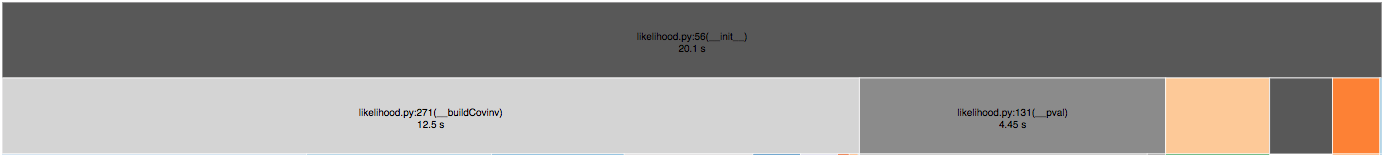
\includegraphics[scale=0.3]{plots/like_after_change_before.png}
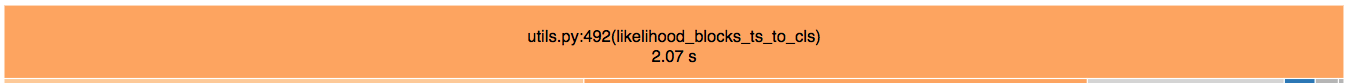
\includegraphics[scale=0.3]{plots/like_ts_to_cls.png}
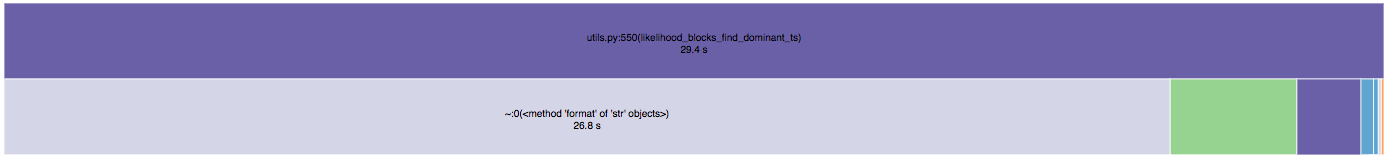
\includegraphics[scale=0.3]{plots/find_dominant_ts_before.png}
\caption{Likelihood object and new functions - Profile after optimisation}
\label{fig:like_last_profile}
\end{figure}

\section{Other Changes}\label{sec:other_changes}
The \texttt{sort\_blocks()} and \classname{likelihood} class optimisations are the two main changes carried out as part of this thesis and the most effective in terms of their reduction of runtime. This section covers two more minor optimisation changes made.

\subsection{Printing Debug Statements}
A large part of the remaining run time in the \classname{Likelihood} object that we see in figure \ref{fig:like_last_profile} comes from the following line of code

\begin{code}
\captionof{listing}{Logging Debug Statements}
\label{code:logging_debug}
\begin{minted}{python}
 contur.config.contur_log.debug(
   "n data, {} signal, {} background {}, bin {} ".format(
    like_ob._n, like_ob._s,  like_ob._bg, like_ob._index))
\end{minted}
\end{code}

In the above each of likelihood objects are numpy arrays and reformatting a large number of these to be printed as strings is time consuming. Further in general the user does not require Contur to print the debug statements in the logger, however in the current set up the reformatting happens regardless whether or not the user has specified to print the strings. The quick fix to this is to place listing \ref{code:logging_debug} within a if statement that only runs if the user specifies to print the debug statements in the logger, this change has been made in listing \ref{code:logging_debug_fix} below.

\begin{code}
\captionof{listing}{Logging Debug Statements With If Statement}
\label{code:logging_debug_fix}
\begin{minted}{python}
if contur.config.contur_log.isEnabledFor(logging.DEBUG):
   contur.config.contur_log.debug(
   "n data, {} signal, {} background {}, bin {} ".format(
   like_ob._n, like_ob._s, like_ob._bg, like_ob._index))
\end{minted}
\end{code}

The impact of this change can be seen in figure \ref{fig:like_last_profile_after_debugger} below. We can see that the change removes much of the remaining runtime in the \classname{Likelihood} object and the \texttt{likelihood\_blocks\_find\_dominant\_ts\_function()} function.

\begin{figure}[H]
\centering
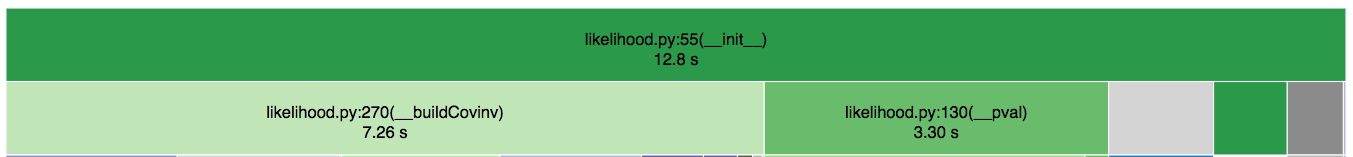
\includegraphics[scale=0.3]{plots/like_after_change.png}

\includegraphics[scale=0.3]{plots/like_blocks_find_dominant_ts.png}
\caption{Likelihood object and new functions - Profile after removing debug print}
\label{fig:like_last_profile_after_debugger}
\end{figure}


\subsection{Strip Options List Concatenation}
In figure \ref{fig:comprehension_before} below we can see a profile for the \texttt{init\_ref()} function, this function deals with the data gathering phase of the Contur run. From the green box in the profile we can see that c.a. 15 seconds of runtime comes from a list comprehension.

\begin{figure}[H]
\centering
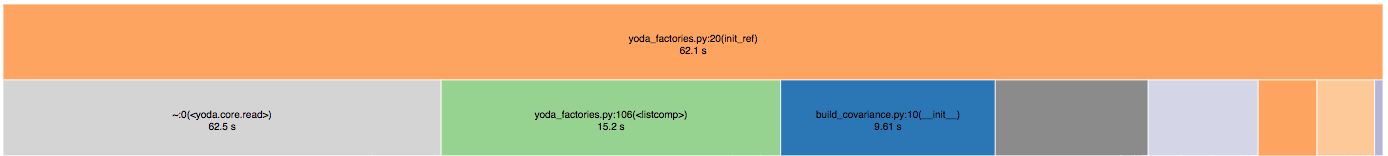
\includegraphics[scale=0.3]{plots/list_comprehension_before.png}
\caption{Likelihood object and new functions - Profile after optimisation}
\label{fig:comprehension_before}
\end{figure}

The specific list comprehension that contributes this 15 seconds is given in listing \ref{code:list_comprehension} below.

\begin{code}
\captionof{listing}{Strip Options List Concatenation}
\label{code:list_comprehension}
\begin{minted}{python}
[match.group() in x for x in 
[rivet.stripOptions(x) for x in aopath]]
\end{minted}
\end{code}

Like other examples we have seen with list comprehensions the extra runtime we get here arises because the list comprehension is placed within another for loop, so the comprehension runs multiple times. In the above it is the inner comprehension that takes up runtime, a simple change we can make is to move this comprehension outside of the for loop and pass the list as a variable in the above line of code in the for loop.

In figure \ref{fig:comprehension_after} below we see the results of this change, namely we get a close to 15 second reduction in run time as we would expect from removing the list comprehension.

\begin{figure}[H]
\centering
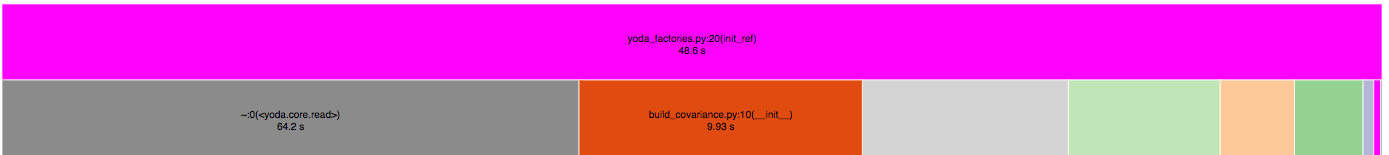
\includegraphics[scale=0.3]{plots/list_comprehension_after.png}
\caption{Likelihood object and new functions - Profile after optimisation}
\label{fig:comprehension_after}
\end{figure}











